% SPDX-License-Identifier: Apache-2.0
% blockpic_in_docs.tex: a sample IEEE two-column document whose figures
% blockpic draws during the Bazel build (collection house style).
\documentclass[journal,9pt]{IEEEtran}
\usepackage{cite}
\usepackage{graphicx}
\usepackage{lmodern}
\usepackage[T1]{fontenc}
\usepackage[utf8]{inputenc}
\usepackage{microtype}
\setlength{\emergencystretch}{3em}
\usepackage{amsmath}
\usepackage{amssymb}
\usepackage{amsthm}
\usepackage{tikz}
\usetikzlibrary{arrows.meta,positioning,fit,calc}
\usepackage{booktabs}
\usepackage{array}
\usepackage{enumitem}
\setlist{nosep,leftmargin=*,topsep=2pt,itemsep=1pt}
\usepackage{float}
\usepackage{xcolor}
\usepackage{listings}
\usepackage[hidelinks,bookmarks=true,pdfauthor={HDL Factory},
            pdftitle={Figures That Follow the Design}]{hyperref}

\theoremstyle{definition}
\newtheorem{guideline}{Guideline}[section]
\newtheorem{example}{Example}[section]
\theoremstyle{remark}
\newtheorem*{tip}{Tip}
\newtheorem*{pitfall}{Pitfall}

\newcommand{\code}[1]{\texttt{#1}}
\newcommand{\term}[1]{\emph{#1}}

% --- Listings: one style per language. The keyword is the only bold role
% and the comment the only italic one, so a listing reads in greyscale.
\definecolor{kwblue}{RGB}{20,60,150}
\definecolor{cmtgreen}{RGB}{90,120,90}
\definecolor{strred}{RGB}{150,50,40}
\definecolor{framegray}{gray}{0.70}
\definecolor{bgshade}{gray}{0.97}

\lstdefinestyle{base}{
  basicstyle=\ttfamily\scriptsize,
  keywordstyle=\bfseries\color{kwblue},
  commentstyle=\itshape\color{cmtgreen},
  stringstyle=\color{strred},
  frame=single,
  rulecolor=\color{framegray},
  framesep=3pt,
  backgroundcolor=\color{bgshade},
  columns=fullflexible,
  keepspaces=true,
  breaklines=true,
  breakatwhitespace=true,
  belowcaptionskip=9pt,
}

\lstdefinelanguage{blockpic}{
  morekeywords={diagram,block,wire,group,layout,kind,name,inputs,outputs,
                params,size,hint,thickness,crossline,at},
  sensitive=true,
  morecomment=[l]{//},
  morestring=[b]",
}

\lstdefinelanguage{starlark}{
  morekeywords={load,def,return,if,else,for,in,True,False,None},
  sensitive=true,
  morecomment=[l]{\#},
  morestring=[b]",
}

\lstdefinestyle{bp}{style=base,language=blockpic}
\lstdefinestyle{bzl}{style=base,language=starlark}
\lstdefinestyle{vlog}{style=base,language=Verilog}

\tikzset{
  box/.style={draw,rounded corners=1pt,align=center,inner sep=3pt,
              minimum height=6.5mm,font=\footnotesize},
  src/.style={box,fill=blue!7},
  act/.style={box,fill=green!12},
  art/.style={box,fill=orange!12},
  fl/.style={-{Stealth[length=4pt]},shorten >=2.5pt,shorten <=2.5pt},
}

% ---------------------------------------------------------------------------
\title{Figures That Follow the Design\\{\large Drawing Block Diagrams and
Netlists with Blockpic in a Bazel Build}}

\author{HDL Factory%
\thanks{A sample document for blockpic, a language and tool that typesets
digital block diagrams. Every figure in it is drawn during the build that
makes this PDF: one from a hand-written diagram, and one from the netlist
that Yosys synthesizes for an AMD 7-series part. The running example is a
4-bit counter that drives four LEDs.}}

\markboth{Blockpic samples~~$\cdot$~~2026}{Figures That Follow the Design}

\begin{document}
\maketitle

\begin{abstract}
A figure in a design document is usually drawn once by hand, and then it
quietly stops matching the design. This sample shows a way to stop that from
happening. Blockpic draws block diagrams from short text files, and it draws
gate-level schematics from the netlists that synthesis writes. A Bazel build
runs synthesis, draws the figures and typesets the document in one graph.
When the HDL changes, the next build redraws the figures. The running
example is a 4-bit LED counter, synthesized by the open AMD 7-series flow of
rules\_openxc7.
\end{abstract}

\begin{IEEEkeywords}
block diagrams, schematics, documentation, netlists, Yosys, Bazel, FPGA
\end{IEEEkeywords}


% SPDX-License-Identifier: Apache-2.0
% 01_intro.tex: Introduction
\section{Introduction}
\label{sec:intro}

\IEEEPARstart{E}{very} design document needs pictures. A reader takes in a
block diagram faster than three paragraphs that say the same thing. The
trouble is that a picture is usually drawn once, in a drawing program, and
saved as an image. The design keeps changing after that, and the picture
does not. A year later, the figure shows a register that was removed and
leaves out the one that replaced it.

Blockpic takes a different approach. A diagram is a short text file, kept in
the repository beside the HDL it describes. The build draws the picture from
that file every time. Blockpic can also draw a picture from the netlist that
synthesis writes, so there is no file to forget at all. When the HDL
changes, the next build redraws the figure from the new netlist.

This document is its own example. Both of its figures were drawn by the
Bazel build that typeset it \cite{bazel}.

\subsection{The running example}

The example design is a 4-bit counter. It adds one to a register on every
rising edge of \code{clk}, clears the register while \code{reset} is high,
and shows the register on four LEDs. Listing~\ref{lst:counter} gives the
whole design.

\lstinputlisting[style=vlog,firstline=4,caption={The running example,
\code{counter.v}.},label={lst:counter},float=t]{counter.v}

The counter is small on purpose. Its schematic after synthesis still fits a
column, and every cell in that schematic can be traced back to a line of the
listing.

\subsection{How to read this document}

Section~\ref{sec:by-hand} draws the counter by hand, in the blockpic
language. Section~\ref{sec:from-netlist} draws the same counter from the
netlist that synthesis writes for an AMD 7-series part. The build that ties
the two to this PDF comes next (\S\ref{sec:build}). The document ends with
what blockpic does not yet do well (\S\ref{sec:limits}).

% SPDX-License-Identifier: Apache-2.0
% 02_by_hand.tex: Drawing a block diagram by hand
\section{Drawing a Block Diagram by Hand}
\label{sec:by-hand}

An architecture diagram shows what a design does, not how synthesis built
it. Someone has to decide what goes in it, so it is written by hand. In
blockpic, it is written as text. Listing~\ref{lst:blockpic} is the counter's
architecture.

\lstinputlisting[style=bp,firstline=6,caption={The counter's architecture,
\code{counter.blockpic}.},label={lst:blockpic},float=t]{counter.blockpic}

A \code{block} has a label, a kind, and its input and output pins. The kind
picks the symbol: \code{ADD} draws an adder, \code{MUX} a multiplexer and
\code{DFF} a flip-flop. A \code{name}, such as \code{+1}, is drawn in place
of the label. An \code{INPUT\_PIN} or
\code{OUTPUT\_PIN} block is a port of the design. A \code{wire} joins an
output pin to an input pin. A wire with a \code{thickness} is drawn as a
bus: a thick line, crossed by a short slash with its width beside it. A
wire can also name the type of the bus, as in \code{type: "nibble\_t"};
the mark then shows the type in place of the width. A \code{group} draws
a dashed box around blocks that belong together, here the counter itself.

\begin{figure}[t]
\centering
\includegraphics[width=\columnwidth]{architecture.pdf}
\caption{The counter's architecture, drawn by blockpic from
Listing~\ref{lst:blockpic}. The thick lines, each marked 4, are the 4-bit buses.}
\label{fig:architecture}
\end{figure}

Fig.~\ref{fig:architecture} is the result. Blockpic placed every block and
routed every wire; the file gives no coordinates. The style is that of the
figures in AMD's UG474 \cite{ug474}: a plain sans-serif face, thin lines
without arrowheads, and pin names such as \code{D} and \code{CK} inside the
box. The feedback from the register to the adder is routed around the
outside, and every 4-bit bus is drawn thick and marked with its width.

\begin{guideline}[Keep the diagram beside the code]
Put the \code{.blockpic} file in the same directory as the HDL it describes.
A change to the design then shows the diagram in the same review, and the
reviewer can ask for the two to agree.
\end{guideline}

\begin{tip}
Name blocks after the signals they make. Here the register is called
\code{count}, as in the Verilog, so a reader can match the figure to the
listing by name.
\end{tip}

% SPDX-License-Identifier: Apache-2.0
% 03_from_netlist.tex: Drawing the netlist that synthesis writes
\section{Drawing the Netlist}
\label{sec:from-netlist}

A hand-drawn diagram shows the intent. The netlist shows what the tools
actually built. The two can differ in ways that matter: a register that
synthesis removed, a bus that got wider, or a carry chain where an adder was
expected. A drawing of the netlist shows those differences directly.

\subsection{From HDL to a JSON netlist}

The counter is synthesized by rules\_openxc7 \cite{rulesopenxc7}, which runs
the open flow for AMD 7-series parts. Yosys \cite{yosys} maps the design to
the part's primitives with \code{synth\_xilinx}. nextpnr \cite{openxc7} and
Project X-Ray \cite{prjxray} then place and route it, but the drawing needs
only the synthesis step. Its output is a JSON netlist: every cell, every
port, and the nets between them, numbered bit by bit.

\subsection{From the netlist to a drawing}

The command \code{blockpic import} reads the netlist and writes a
\code{.blockpic} file. From there, the netlist is drawn in exactly the same
way as Fig.~\ref{fig:architecture}. Table~\ref{tab:mapping} lists how each
part of the netlist is drawn.

\begin{table}[t]
\centering
\caption{How \code{blockpic import} draws a netlist.}
\label{tab:mapping}
\footnotesize
\begin{tabular}{@{}>{\raggedright}p{0.38\columnwidth}
                >{\raggedright\arraybackslash}p{0.54\columnwidth}@{}}
\toprule
In the netlist & In the drawing \\
\midrule
A cell, such as \code{FDRE} & A block of that kind \\
A module port & An input or output port block \\
A bus that goes whole to one pin & One thick wire \\
A bus whose bits go apart & A pin per bit, such as \code{O\_1} \\
A constant 0 or 1 & A \code{GND} or \code{VCC} block \\
Any other constant & A \code{CONST} block with its value \\
\bottomrule
\end{tabular}
\end{table}

\begin{figure*}[t]
\centering
\includegraphics[width=0.72\textwidth]{netlist.pdf}
\caption{The counter after synthesis for the xc7a200t, drawn by blockpic
from the netlist that Yosys wrote.}
\label{fig:netlist}
\end{figure*}

\subsection{Reading the drawing}

Fig.~\ref{fig:netlist} is the counter as Yosys built it. Each part of
Listing~\ref{lst:counter} can be found in it:
\begin{itemize}
\item The register is four \code{FDRE} flip-flops, one per bit. Each is
  drawn as a box with its pin names inside, as UG474 draws one. Their
  \code{R} pins are the synchronous reset, and \code{CE} is tied to
  \code{VCC}.
\item The adder became one \code{CARRY4}, the carry chain of a 7-series
  slice \cite{ug474}. Its \code{O\_1} to \code{O\_3} outputs feed the upper
  three flip-flops. Bit 0 needs no adder: an \code{INV} toggles it.
\item Every port went through a buffer: \code{IBUF} on \code{clk} and
  \code{reset}, \code{OBUF} on each LED. The clock also goes through a
  \code{BUFG} onto the global clock network.
\item The bus \code{led} was split into \code{led\_0} to \code{led\_3},
  because each bit leaves through its own buffer.
\end{itemize}

None of this is in the hand-drawn Fig.~\ref{fig:architecture}, and none of it
should be. The two figures answer different questions. The architecture
says what the counter does. The netlist says what the FPGA will run.

\begin{pitfall}
A netlist drawing grows with the design. A counter fits a column, but a
processor gives thousands of cells and an unreadable picture. Synthesis for
the FPGA also flattens the design into one module. To draw one part of a
large design, synthesize that part on its own, with it as the top level.
\end{pitfall}

% SPDX-License-Identifier: Apache-2.0
% 04_build.tex: One build from HDL to PDF
\section{One Build from HDL to PDF}
\label{sec:build}

The figures stay current because nobody draws them. Bazel \cite{bazel}
builds them from their sources, like any other output. Fig.~\ref{fig:graph}
shows the build graph behind this document.

\begin{figure}[!tb]
\centering
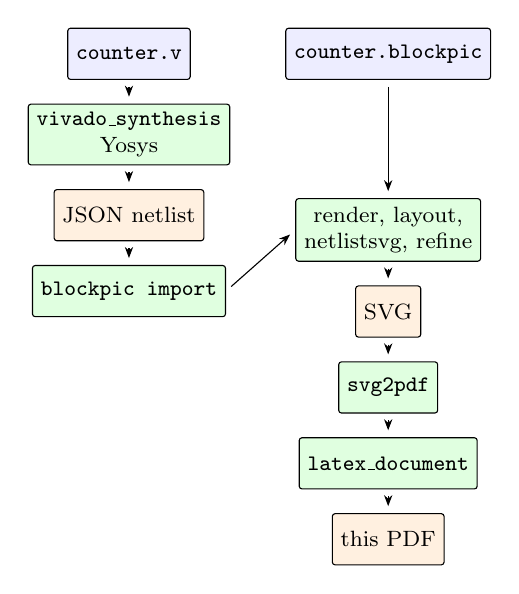
\begin{tikzpicture}[node distance=3mm and 3mm,
  every node/.append style={font=\scriptsize,minimum height=5mm}]
  \node[src] (v) {\code{counter.v}};
  \node[act, below=of v] (syn) {\code{vivado\_synthesis}\\Yosys};
  \node[art, below=of syn] (json) {JSON netlist};
  \node[act, below=of json] (imp) {\code{blockpic import}};
  \node[src, right=12mm of v] (bp) {\code{counter.blockpic}};
  \node[act, below=15mm of bp] (draw) {render, layout,\\netlistsvg, refine};
  \node[art, below=of draw] (svg) {SVG};
  \node[act, below=of svg] (pdf) {\code{svg2pdf}};
  \node[act, below=of pdf] (tex) {\code{latex\_document}};
  \node[art, below=of tex] (out) {this PDF};
  \draw[fl] (v) -- (syn);
  \draw[fl] (syn) -- (json);
  \draw[fl] (json) -- (imp);
  \draw[fl] (imp.east) -- (draw.west);
  \draw[fl] (bp) -- (draw);
  \draw[fl] (draw) -- (svg);
  \draw[fl] (svg) -- (pdf);
  \draw[fl] (pdf) -- (tex);
  \draw[fl] (tex) -- (out);
\end{tikzpicture}
\caption{The build graph of this document. Blue boxes are sources, green
boxes are build steps, and orange boxes are their outputs. Both figures
take the right-hand path.}
\label{fig:graph}
\end{figure}

Each box in the figure is one target, or one step inside a target.
Listing~\ref{lst:build} shows the targets in this document's
\code{BUILD.bazel} that draw the netlist figure.
\code{blockpic\_netlist\_diagram} takes any target whose only output is a
Yosys JSON netlist. \code{vivado\_synthesis} is one such target.

\begin{lstlisting}[style=bzl,float=t,caption={The targets that draw
Fig.~\ref{fig:netlist}.},label={lst:build}]
vivado_project(
    name = "counter",
    srcs = ["counter.v"],
    part = "xc7a200tfbg484-2",
    top_level = "counter",
)

vivado_synthesis(
    name = "counter_synth",
    project = ":counter",
)

blockpic_netlist_diagram(
    name = "netlist",
    netlist = ":counter_synth",
    out = "netlist.svg",
)

svg_to_pdf(
    name = "netlist_pdf",
    src = ":netlist",
    out = "netlist.pdf",
)
\end{lstlisting}

The document target lists \code{:netlist\_pdf} among its inputs. So when
\code{counter.v} changes, Bazel synthesizes the design again, redraws the
figure and typesets the PDF again. When nothing changed, Bazel reuses all
three results from its cache.

\subsection{Turning SVG into PDF}

pdflatex cannot include an SVG. \code{svg2pdf} converts each drawing into a
one-page PDF of the same size, a pixel taken as a point. It embeds its font,
DejaVu Sans, because a PDF for print must carry every font it uses.
The converter is a short Node.js script, built from pinned npm packages, so
the conversion is the same on every machine.

\subsection{Publishing}

A scheduled workflow builds this document and publishes it on the
repository's release page. The same workflow attaches it to every tagged
release of blockpic. A reader of a release therefore gets the figures drawn
by that release's code.

\begin{guideline}[Let the build own the figures]
Never commit a generated figure. Commit its source, the \code{.blockpic}
file or the HDL, and let the build draw it. A committed image is one more
file that can fall behind.
\end{guideline}

% SPDX-License-Identifier: Apache-2.0
% 05_limits.tex: What blockpic does not do yet
\section{What Blockpic Does Not Do Yet}
\label{sec:limits}

Blockpic is young, and both figures in this document show where.

\begin{itemize}
\item \textbf{Layout.} ELK places every block. It cannot be told to
  line the four flip-flops up in a column, which a person drawing
  Fig.~\ref{fig:netlist} would do. Wires that fan out, such as the clock
  and the reset, still bend on their way to each flip-flop.
\item \textbf{Size.} A netlist of a few dozen cells is readable. One of a
  few thousand is not, so draw small modules (\S\ref{sec:from-netlist}).
\end{itemize}

% SPDX-License-Identifier: Apache-2.0
% 06_conclusion.tex: Conclusion
\section{Conclusion}
\label{sec:conclusion}

A figure that the build draws cannot fall behind the design. This document
showed two kinds. An architecture diagram is written by hand in a few lines
of text and kept beside the HDL. A netlist drawing needs no source of its
own, because synthesis writes it. Bazel ties both to the document, so a
change to \code{counter.v} reaches Fig.~\ref{fig:netlist} in the next build.

To start, write a \code{.blockpic} file for one block diagram in an
existing document, and add the targets of Listing~\ref{lst:build} to its
build. The figure then stays correct for as long as the build passes.


% =====================================================================
\begin{thebibliography}{10}
\bibitem{yosys} C.~Wolf, ``Yosys Open SYnthesis Suite,''
  \url{https://yosyshq.net/yosys/}.
\bibitem{netlistsvg} N.~Turley, ``netlistsvg: draws an SVG schematic from a
  Yosys JSON netlist,'' \url{https://github.com/nturley/netlistsvg}.
\bibitem{openxc7} openXC7, ``nextpnr for AMD 7-series FPGAs, the himbaechel
  Xilinx architecture,'' \url{https://github.com/openXC7/nextpnr}.
\bibitem{prjxray} F4PGA, ``Project X-Ray: documenting the 7-series
  bitstream format,'' \url{https://github.com/f4pga/prjxray}.
\bibitem{rulesopenxc7} F.~Filmar, ``rules\_openxc7: Bazel rules for AMD
  7-series FPGAs with the open toolchain,''
  \url{https://github.com/filmil/bazel_rules_openxc7}.
\bibitem{ug474} AMD, ``7 Series FPGAs Configurable Logic Block User
  Guide,'' UG474.
\bibitem{bazel} The Bazel Authors, ``Bazel,'' \url{https://bazel.build}.
\end{thebibliography}

\end{document}
